
\section{講義概要}


\begin{frame}
\frametitle{今日の内容}


前回に引き続いてテイラーの定理に関する話題を議論する. 
\begin{enumerate}
\item テイラーの定理の証明
\item テイラー展開, 解析的関数
\item 応用, オイラーの公式
\item 収束半径
\end{enumerate} 



\end{frame}


\begin{slide}{整級数・テイラー展開・マクローリン展開}
\begin{itemize}
\item 多項式近似の係数を求めるために整級数(power series)を用いる\footnote{整級数は、「多項式関数で表す」と等価である}
\item 与えられた関数を指定した値$a$の付近の整級数で表すことをテイラー展開(Taylor expansion)、$a=0$の時マクローリン展開(Maclaurin expansion)\footnote{マクローラン展開と訳されることもある}とよび、その時使う級数をテイラー級数(Taylor series)、マクローリン級数(Maclaurin series)と呼ぶ。
\item 基本原理はテイラーの定理(Taylor's theorem)である
\end{itemize}
\end{slide}
\begin{slide}{5.2 [2] テイラー展開}
\begin{itemize}
\item 与えられた関数$f(x)$を定数$a$を中心にして、多項式近似したものがテイラー展開である。
\begin{equation}
f(x) \approx f(a) + f'(a)(x-a) + \frac{1}{2!}f''(a)(x-a)^2 + \frac{1}{3!}f'''(a)(x-a)^3 + \cdots \label{eq:taylorseries}
\end{equation}
\item テイラー展開において$a=0$の場合、マクローリン展開と呼ばれる。
\begin{equation}
f(x) \approx f(0) + f'(0)(x) + \frac{1}{2!}f''(0)(x)^2 + \frac{1}{3!}f'''(0)(x)^3 + \cdots \label{eq:macseries}
\end{equation}
\end{itemize}
\end{slide}
\begin{slide}{テイラー展開の導出}
\begin{itemize}
\item 与えられた関数が次のように多項式で近似できるとし、$a$を中心に$a_0, a_1, \cdots$を求める。
\begin{equation}
f(x) =  a_0 + a_1 x + a_2x^2 + a_3 x^3 + a_4x^4 +\cdots \label{eq:taylor}
\end{equation}
$x=a$では以下が成立。
\begin{equation}
f(a) =  a_0 + a_1 a + a_2a^2 + a_3 a^3 + a_4a^4 +\cdots  \nonumber 
\end{equation}
高次導関数は以下のように求められる。係数が次数に応じた階乗になることに注目。
\begin{eqnarray}
f'(x) &=& a_1 + 2a_2x+ 3a_3 x^2 + 4a_4x^3+\cdots \nonumber \\
f''(x) &=& 2a_2 + 6a_3 x + 12 a_4x^2 + \cdots \nonumber \\
f'''(x) &=& 6a_3 + 24 a_4 x + \cdots \nonumber \\
\vdots \label{eq:higherderivatives}
\end{eqnarray}
\end{itemize}
\end{slide}
\begin{slide}{テイラー展開の導出2}
\begin{itemize}
\item 式\ref{eq:taylor}に$x=a+h$を代入すると
\begin{eqnarray}
f(a+h) &=& a_0 + a_1 (a+h) + a_2 (a+h)^2 + a_3 (a+h)^3 +  \cdots \nonumber \\
&=& a_0 + a_1 a + a_2 a^2 + a_3 a^3 + a_4 a^4 + \cdots \nonumber \\
&+& h(a_1 + 2a_2a + 3a_3a^2 + 4a_4a^3 + \cdots \nonumber \\
&+& h^2(a_2 + 3a_3a + 6a_4 a^2 + \cdots \nonumber \\
&+& h^3(a_3 + 4a_4a + \cdots \nonumber 
\end{eqnarray}
\item 式\ref{eq:higherderivatives}の高次導関数を用いると
\begin{eqnarray}
f(a+h) &=& a_0 + a_1 (a+h) + a_2 (a+h)^2 + a_3 (a+h)^3 +  \cdots \nonumber \\
&=& f(a) +  hf'(a) + \frac{h^2}{2!}f''(a) + \frac{h^3}{3!}f'''(a) + \cdots  \nonumber
\end{eqnarray}
$h=x-a$なのでテイラー展開(式\ref{eq:taylorseries})を得る。$a=0$ならマクローリン展開(式\ref{eq:macseries})である。
\end{itemize}  
\end{slide}
\begin{slide}{例題 5.2}
次の関数をマクローリン展開を用いて三次式で近似せよ。
\begin{itemize}
\item $\sin{x}$ 
\begin{eqnarray}
\sin{x} &\approx& \sin{0}  + \cos{0}x -\frac{1}{2}\sin{0}x^2- \frac{1}{6}\cos{0}x^3 \nonumber  \\
&=& x - \frac{1}{6}x^3 
\end{eqnarray}
\item $\log_e{(x+1)}$
\begin{eqnarray}
\log_e{(x+1)} &\approx& \log_e{1} + \frac{1}{0+1} x - \frac{1}{2}\frac{1}{(0+1)^2} x^2 +\frac{2}{6} \frac{1}{(1+0)^3} x^3 \nonumber \\
&=& x - \frac{1}{2}x^2 + \frac{1}{3}x^3\nonumber 
\end{eqnarray}
\end{itemize}
\end{slide}
\begin{slide}{例題5.2の図解}
\begin{figure}[h]
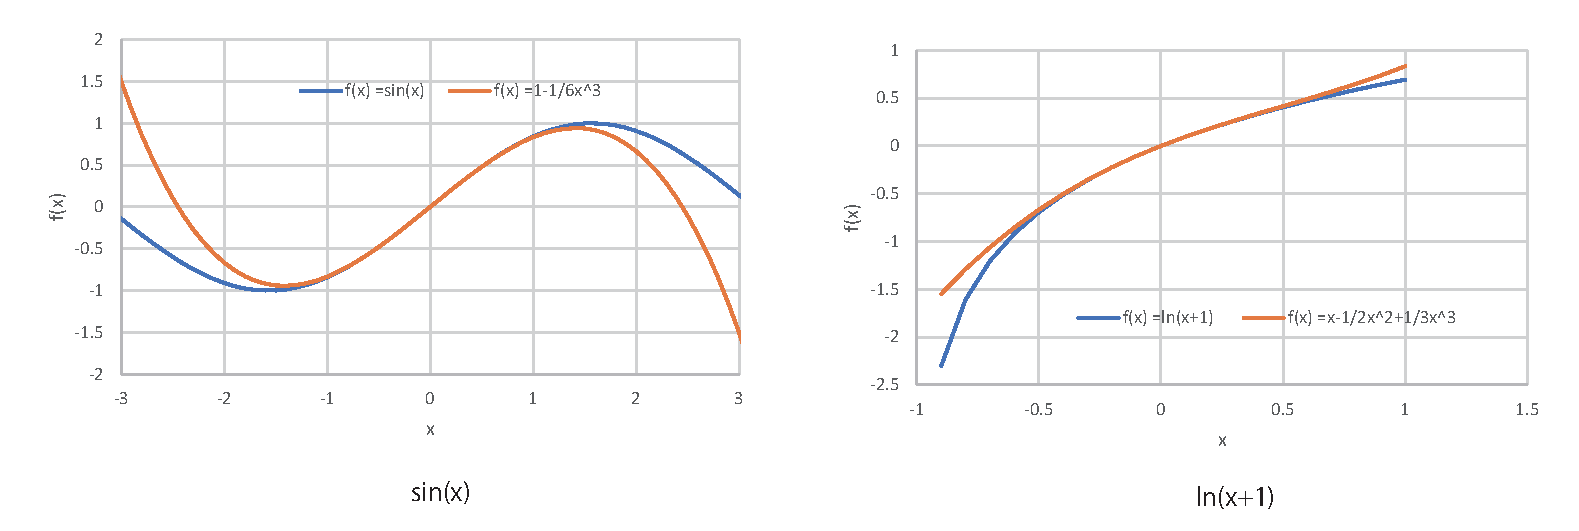
\includegraphics[width=11cm]{calculus9/macapx.eps}
\end{figure}
\end{slide}
\begin{slide}{問題 5.2}
次の関数をマクローリン展開を用いて三次式で近似せよ。
\begin{itemize}
\item $\frac{1}{x+1}$
\item $\sqrt{x+1}$
\end{itemize}
\end{slide}
\begin{slide}{[3]テイラーの定理:参考}
\begin{itemize}
\item 関数$f(x)$が$C^{n+1}$級で区間$a \leqq x \leqq b$が$f(x)$の定義域に含まれていれば$h=b-a$として
\begin{eqnarray}
f(b) &=& f(a) + f'(a)h+\frac{1}{2!}f''(a)h^2 + \cdots \nonumber \\
&+& \frac{1}{n!}f^{(n)}(a)h^n + \frac{1}{(n+1)!}f^{(n+1)}(c)(h)^{n+1} \nonumber \\
&=& f(a) + \sum_{i=1}^n \frac{1}{i!}f^{(i)} (a)h^i +  \frac{1}{(n+1)!}f^{(n+1)}(c)(h)^{n+1} \nonumber
\end{eqnarray}
となる$c$が$a$と$b$の間に少なくとも一つ存在する。
\item 証明:テイラー級数を$f^{(n)}$の項で打ち切った場合と考え、次の$g(x)$を導入する。
\begin{equation}
g(x) =  f(x) +  \sum_{i=1}^n \frac{1}{i!}f^{(i)}(x) (b-x)^i  + K(b-x)^{n+1}   \nonumber
\end{equation}
\end{itemize}
\end{slide}
\begin{slide}{[3]テイラーの定理:参考2}
\begin{itemize}
\item $K$を次式が成立するように決定する。
\begin{equation}
g(a) = f(a) + \sum_{i=1}^n \frac{1}{i!}f^{(i)}(a) (b-a)^i  + K(b-a)^{n+1} = f(b) \nonumber 
\end{equation}
具体的には$K$は以下である。
\begin{equation}
K = \frac{f(b) - f(a) - \sum_{i=1}^n \frac{1}{i!}f^{(i)}(a)(b-a)^i }{(b-a)^{n+1}} \label{eq:taylortheorem}
\end{equation}
$x=b$の時は式の定義により明らかに$g(b) = f(b)$である。
\end{itemize}
\end{slide}
\begin{slide}{[3]テイラーの定理:参考3}
\begin{itemize}
\item このように$K$を決めることで$g(a)=g(b)=f(b)$なのでロールの定理(7回参照)により$g'(c)=0$となる$c$が$a<c<b$に少なくとも一つ存在する。
\begin{eqnarray}
&& g'(x) = f'(x) \nonumber  \\
&+& \sum_{i=1}^n \frac{1}{i!}f^{(i+1)}(x)(b-x)^i - \frac{i}{i!}f^{(i)}(x)(b-x)^{i-1} \nonumber \\
&-& (n+1)K(b-x)^{n} \nonumber
\end{eqnarray}
なので$x=c$の時
\begin{eqnarray}
&& g'(c) = f'(c) \nonumber \\
 &+& \sum_{i=1}^n \frac{1}{i!}f^{(i+1)}(c)(b-c)^i - \frac{1}{(i-1)!}f^{(i)}(c)(b-c)^{i-1} \nonumber \\
 &-& (n+1)K(b-c)^{n} = 0 \nonumber
\end{eqnarray}
\end{itemize}
\end{slide}
\begin{slide}{[3]テイラーの定理:参考4}
\begin{itemize}
\item 総和の中は次のようにほとんど打消される。
\begin{eqnarray}
&&\sum_{i=1}^n \frac{1}{i!}f^{(i+1)}(c)(b-c)^i - \frac{1}{(i-1)!}f^{(i)}(c)(b-c)^{i-1} \nonumber \\
&=& \cancel{f^{(2)}(c)(b-c)} - f'(c) \nonumber \\
&& + \cancel{\frac{1}{2}f^{(3)}(c)(b-c)^2}  - \cancel{f^{(2)}(c)(b-c)} \nonumber \\
&& + \cancel{\frac{1}{3!}f^{(4)}(c)(b-c)^3} - \cancel{\frac{1}{2}f^{(3)}(c)(b-c)^2} \nonumber \\
&& \vdots \nonumber \\
&& + \frac{1}{n!}f^{(n+1)}(c)(b-c)^n- \cancel{\frac{1}{(n-1)!}f^{(n)}(c)(b-c)^{n-1}} \nonumber \\
&=&  \frac{1}{n!}f^{(n+1)}(c)(b-c)^n - f'(c) \label{eq:taylorsum}
\end{eqnarray}
\end{itemize}
\end{slide}
\begin{slide}{[3]テイラーの定理:参考5}
\begin{itemize}
\item 式\ref{eq:taylorsum}を用いて$g'(c)$を書き直すと
\begin{equation}
g'(c) = \cancel{f'(c)} + \frac{1}{n!}f^{(n+1)}(c)(b-c)^n - \cancel{f'(c)} - (n+1)K(b-c)^{n} = 0 \nonumber 
\end{equation}
\item したがって
\begin{equation}
K = \frac{1}{(n+1)!}f^{(n+1)}(c) \nonumber 
\end{equation}
となり、式\ref{eq:taylortheorem}に代入して
\begin{equation}
K = \frac{f(b) - f(a) - \sum_{i=1}^n \frac{1}{i!}f^{(i)}(a)(b-a)^i }{(b-a)^{n+1}}  = \frac{1}{(n+1)!}f^{(n+1)}(c) \nonumber
\end{equation}
\item 式を変形するとテイラーの定理が得られる。
\begin{equation}
f(b) = f(a) + \sum_{i=1}^n \frac{1}{i!}f^{(i)}(a)(b-a)^i  + \frac{(b-a)^{n+1}}{(n+1)!}f^{(n+1)}(c) \nonumber
\end{equation}
\end{itemize}
\end{slide}
\begin{slide}{[4]ロピタルの定理:テーラー展開による導出}
\begin{itemize}
\item 極限$\lim_{x \to a}\frac{f(x)}{g(x)}$が$\frac{0}{0}$または$\pm\frac{\infty}{\infty}$の時、極限$\lim_{x\to a}\frac{f'(x)}{g'(x)}$が確定した値に収束すれば
\begin{equation}
\lim_{x\to a} \frac{f(x)}{g(x)} = \lim_{x\to a}\frac{f'(x)}{g'(x)}
\end{equation}
が成り立つ。
\item 証明:$f(x), g(x)$が$x=a$でゼロの場合、$a$付近でテイラー展開すると
\begin{eqnarray}
f'(x) &=& f(a) + f'(a) (x-a) + \frac{1}{2}f''(a)(x-a)^2 + \cdots \nonumber \\
g(x) &=& g(a) + g'(a)(x-a) +  \frac{1}{2}g''(a)(x-a)^2 + \cdots \nonumber
\end{eqnarray}
となる。
\end{itemize}
\end{slide}





%%%%%%%%%%%%%%%%%%%%%%%%%%%%%%%%%%%%%%%%%%%%%%%%%%%%%%%%%%%%%%%%%%%%%%%%%%%%%%%%%%%%%%%
%%%%%%%%%%%%%%%%%%%%%%%%%%%%%%%%%%%%%%%%%%%%%%%%%%%%%%%%%%%%%%%%%%%%%%%%%%%%%%%%%%%%%%%





%%%%%%%%%%%%%%%%%%%%%%%%%%%%%%%%%%%%%%%%%%%%%%%%%%%%%%%%%%%%%%%%%%%%%%%%%%%%%%%%%%%%%%%
%%%%%%%%%%%%%%%%%%%%%%%%%%%%%%%%%%%%%%%%%%%%%%%%%%%%%%%%%%%%%%%%%%%%%%%%%%%%%%%%%%%%%%%





%%%%%%%%%%%%%%%%%%%%%%%%%%%%%%%%%%%%%%%%%%%%%%%%%%%%%%%%%%%%%%%%%%%%%%%%%%%%%%%%%%%%%%%
%%%%%%%%%%%%%%%%%%%%%%%%%%%%%%%%%%%%%%%%%%%%%%%%%%%%%%%%%%%%%%%%%%%%%%%%%%%%%%%%%%%%%%%



\begin{frame}
\frametitle{$e^x$のマクローリン展開}

$f(x)=e^x$に関して, $f^{(n)}(x)=e^x$であるから, 有限マクローリン展開は
$$
e^x=1+x+\frac{x^2}{2!}+\frac{x^3}{3!}+\dots+\frac{x^{n-1}}{(n-1)!}+\frac{e^{\theta x}}{n!}x^n. 
$$
ただし$0<\theta < 1$. 
任意の$x$に対して
$$
\frac{e^{\theta x}}{n!}x^n \to 0 \ \ \ (n \to \infty) 
$$
であるから\footnote{次ページで証明}, $f(x)=e^x$のマクローリン展開は
$$
e^x= \sum_{k=0}^{\infty}\frac{x^k}{k!}
=1+x+\frac{x^2}{2!}+\frac{x^3}{3!}+\dots
$$
簡単のため, $0<x$としたが, $0>x$でも成立する.  
\end{frame}



%%%%%%%%%%%%%%%%%%%%%%%%%%%%%%%%%%%%%%%%%%%%%%%%%%%%%%%%%%%%%%%%%%%%%%%%%%%%%%%%%%%%%%%
%%%%%%%%%%%%%%%%%%%%%%%%%%%%%%%%%%%%%%%%%%%%%%%%%%%%%%%%%%%%%%%%%%%%%%%%%%%%%%%%%%%%%%%
\begin{slide}{$\sum_{n = 0}^{\infty} \frac{x^n}{n!} = 0$の証明}
$n$は無限大まで大きくなるため、任意の$|x|$よりも大きくなる$N$を選ぶことができる。その場合
\begin{equation}
\sum_{n= 0}^{\infty} \frac{x^n}{n!} = \sum_{n = 0}^{N-1} \frac{x^n}{n!} + \sum_{n=N}^{\infty}\frac{x^n}{n!} \nonumber
\end{equation}
である。第一項は有限和なので必ず収束する。第2項は自然数$i$を用いて$n=N+i $と書き直すと、$n! = (N+i)(N+i-1) \cdots (N+1) N! $なので、$n! > N^i N!$である。したがって
\begin{equation}
 \sum_{n=N}^{\infty}\frac{x^n}{n!} < \frac{x^N}{N!}\sum_{i=0}^\infty \frac{x^i}{N^i} \nonumber
\end{equation}
となり$x/N<1$より、上式はゼロに収束する\footnote{後の講義で説明する収束半径を用いるとより直観的に証明できる}. 
\end{slide}


\begin{frame}
\frametitle{$\sin x$のマクローリン展開}

$f(x)=\sin x$の有限マクローリン展開を求める. 
$$
f'(x)=\cos x, \ f^{(2)}(x)=-\sin x, \ f^{(3)}(x)=-\cos x, \ f^{(4)}(x)=\sin x
$$
を周期$4$で繰り返すことから
$$
 f^{(4n)}(0)=0, \ f^{(4n+1)}(0)=1, \ f^{(4n+2)}(0)=0, \ f^{(4n+3)}(0)=-1. 
$$
したがって
\begin{align*}
\sin x & = \sum_{k=0}^{n-1}(-1)^k\frac{x^{2k+1}}{(2k+1)!}+R \\
& = x-\frac{x^3}{3!}+\frac{x^5}{5!}+\dots+\frac{(-1)^{n-1}}{(2n-1)!}x^{2n-1}+R
\end{align*}
	

\end{frame}




%%%%%%%%%%%%%%%%%%%%%%%%%%%%%%%%%%%%%%%%%%%%%%%%%%%%%%%%%%%%%%%%%%%%%%%%%%%%%%%%%%%%%%%
%%%%%%%%%%%%%%%%%%%%%%%%%%%%%%%%%%%%%%%%%%%%%%%%%%%%%%%%%%%%%%%%%%%%%%%%%%%%%%%%%%%%%%%



\begin{frame}
\frametitle{$\sin x$のマクローリン展開}

ただし, 剰余項$R$は$R_{2n}$または$R_{2n+1}$であり, ある$0 < \theta <1$に関して
$$
R_{2n}=\frac{(-1)^n \sin(\theta x)}{(2n)!}x^{2n}, \ \ \ R_{2n+1}=\frac{(-1)^n \cos(\theta x)}{(2n+1)!}x^{2n+1}. 
$$
いずれの場合も
$$
|R_N| \le \frac{x^N}{N!} \to 0 \ \ \ (N \to \infty) 
$$
であるから, $f(x)=\sin x$のマクローリン展開は
\begin{align*}
\sin x & = \sum_{k=0}^{\infty}(-1)^k\frac{x^{2k+1}}{(2k+1)!} \\
& = x-\frac{x^3}{3!}+\frac{x^5}{5!}-\frac{x^7}{7!}+\dots 
\end{align*}

\end{frame}


%%%%%%%%%%%%%%%%%%%%%%%%%%%%%%%%%%%%%%%%%%%%%%%%%%%%%%%%%%%%%%%%%%%%%%%%%%%%%%%%%%%%%%%
%%%%%%%%%%%%%%%%%%%%%%%%%%%%%%%%%%%%%%%%%%%%%%%%%%%%%%%%%%%%%%%%%%%%%%%%%%%%%%%%%%%%%%%



\begin{frame}
\frametitle{$\cos x$のマクローリン展開}

$f(x)=\cos x$のマクローリン展開も同様に求めることができる. 

\begin{align*}
\cos x & = \sum_{k=0}^{\infty}(-1)^k\frac{x^{2k}}{(2k)!} \\
& = 1-\frac{x^2}{2!}+\frac{x^4}{4!}-\frac{x^6}{6!}+\dots 
\end{align*}

これらのマクローリン展開からも, $(\sin x)'=\cos x$, $(\cos x)' = -\sin x$が成立していることが分かる. (項別微分)

\end{frame}


%%%%%%%%%%%%%%%%%%%%%%%%%%%%%%%%%%%%%%%%%%%%%%%%%%%%%%%%%%%%%%%%%%%%%%%%%%%%%%%%%%%%%%%
%%%%%%%%%%%%%%%%%%%%%%%%%%%%%%%%%%%%%%%%%%%%%%%%%%%%%%%%%%%%%%%%%%%%%%%%%%%%%%%%%%%%%%%



%\begin{frame}
%\frametitle{三角関数と弧度法}
%
%解析学において, 三角関数を弧度法で考えることは重要である. 
%実際, 度数法の世界では三角関数の基本的な公式は複雑になる($1^\circ=\frac{\pi}{180}$rad):  
%\begin{itemize}
%\item $\displaystyle \lim_{x\to0}\frac{\sin x}{x}=\frac{\pi}{180}$
%\item $\displaystyle (\sin x)'=\frac{\pi}{180} \cos x, \ \ \  (\cos x)'=-\frac{\pi}{180} \sin x$
%\item $\displaystyle \sin x = \frac{\pi}{180} x - \frac{\pi^3}{180^3}\frac{x^3}{3!}+\frac{\pi^5}{180^5}\frac{x^5}{5!}+\dots$
%\end{itemize}
%弧度法では形式的にラジアンという単位を使うが, 実際は円の半径と弧の比であるから(長さの単位に依存しない)無次元量である. 
%本来, 数は無次元量であり, それゆえ$x+x^3$のような計算が意味を持つのである. 
%
%\end{frame}


%%%%%%%%%%%%%%%%%%%%%%%%%%%%%%%%%%%%%%%%%%%%%%%%%%%%%%%%%%%%%%%%%%%%%%%%%%%%%%%%%%%%%%%
%%%%%%%%%%%%%%%%%%%%%%%%%%%%%%%%%%%%%%%%%%%%%%%%%%%%%%%%%%%%%%%%%%%%%%%%%%%%%%%%%%%%%%%



\begin{frame}
\frametitle{$\frac{1}{1-x}$のマクローリン展開}

$f(x)=\frac{1}{1-x}$の有限マクローリン展開を求める. 
\begin{align*}
f'(x)=\frac{1}{(1-x)^2}, \ \ \ f''(x)=\frac{2}{(1-x)^3}, \ \ \  f^{(3)}(x)=\frac{3\cdot 2}{(1-x)^4}, \dots 
\end{align*}
であり, 一般に$f^{(k)}(x)=\frac{k!}{(1-x)^{k+1}}$であるから
\begin{align*}
\frac{1}{1-x} & = \sum_{k=0}^{n-1}x^k+\frac{1}{(1-\theta x)^{n+1}}x^n \\
& = 1+x+x^2+\dots+x^{n-1}+\frac{1}{(1-\theta x)^{n+1}}x^n
\end{align*}
ただし$0<\theta < 1$. 

\end{frame}

%%%%%%%%%%%%%%%%%%%%%%%%%%%%%%%%%%%%%%%%%%%%%%%%%%%%%%%%%%%%%%%%%%%%%%%%%%%%%%%%%%%%%%%
%%%%%%%%%%%%%%%%%%%%%%%%%%%%%%%%%%%%%%%%%%%%%%%%%%%%%%%%%%%%%%%%%%%%%%%%%%%%%%%%%%%%%%%



\begin{frame}
\frametitle{$\frac{1}{1-x}$のマクローリン展開}

$-1 < x < 1$であれば
$$
\frac{|x|^n}{|1-\theta x|^{n+1}} \le \frac{|x|^n}{|1-|x||^{n+1}} \to 0 \ \ \ (n\to \infty)
$$
であるから, $\frac{1}{1-x}$のマクローリン展開は
\begin{align*}
\frac{1}{1-x} & = \sum_{k=0}^{\infty} x^k \\
&=1+x+x^2+x^3+x^4+\dots. 
\end{align*}
実際には, $-1<x<1$においてマクローリン展開が成立する. 
(等比数列の和と思えば良い.)

\end{frame}




%%%%%%%%%%%%%%%%%%%%%%%%%%%%%%%%%%%%%%%%%%%%%%%%%%%%%%%%%%%%%%%%%%%%%%%%%%%%%%%%%%%%%%%
%%%%%%%%%%%%%%%%%%%%%%%%%%%%%%%%%%%%%%%%%%%%%%%%%%%%%%%%%%%%%%%%%%%%%%%%%%%%%%%%%%%%%%%



\begin{frame}
\frametitle{$\log(1+x)$のマクローリン展開}

$f(x)=\log(1+x)$の有限マクローリン展開を求める. 
\begin{align*}
f'(x)=\frac{1}{1+x}, \ \ \  f''(x)=\frac{-1}{(1+x)^2}, \ \ \  f^{(2)}(x)=\frac{2}{(1+x)^3}, \dots
\end{align*}
であり, 一般に$f^{(k)}(x)=\frac{(-1)^{k+1}(k-1)!}{(1+x)^{k}}$であるから
\begin{align*}
\log(1+x) &= \sum_{k=1}^{n-1}(-1)^{k+1}\frac{x^k}{k}+\frac{(-1)^{n+1}}{n(1+\theta x)^{n}}x^n \\
& = x-\frac{x^2}{2}+\frac{x^3}{3}+ \dots +(-1)^{n}\frac{x^{n-1}}{n-1}+\frac{(-1)^{n+1}}{n(1+\theta x)^{n}}x^n. 
\end{align*}
ただし$0<\theta < 1$. 

\end{frame}




%%%%%%%%%%%%%%%%%%%%%%%%%%%%%%%%%%%%%%%%%%%%%%%%%%%%%%%%%%%%%%%%%%%%%%%%%%%%%%%%%%%%%%%
%%%%%%%%%%%%%%%%%%%%%%%%%%%%%%%%%%%%%%%%%%%%%%%%%%%%%%%%%%%%%%%%%%%%%%%%%%%%%%%%%%%%%%%


\begin{frame}
\frametitle{$\log(1+x)$のマクローリン展開}

$0\le x\le 1$であれば
$$
\frac{|(-1)^{n+1}x^n|}{|n(1+\theta x)^{n}|} \le \frac{1}{n} \to 0 \ \ \ (n\to \infty)
$$
であるから, $\log(1+x)$のマクローリン展開は
\begin{align*}
\log(1+x) & =  \sum_{k=1}^{\infty}(-1)^{k+1}\frac{x^k}{k} \\
& =  x-\frac{x^2}{2}+\frac{x^3}{3} - \frac{x^4}{4}+\dots.
\end{align*}
実際は, $-1<x<1$においてマクローリン展開が成立する. 

\end{frame}

%%%%%%%%%%%%%%%%%%%%%%%%%%%%%%%%%%%%%%%%%%%%%%%%%%%%%%%%%%%%%%%%%%%%%%%%%%%%%%%%%%%%%%%
%%%%%%%%%%%%%%%%%%%%%%%%%%%%%%%%%%%%%%%%%%%%%%%%%%%%%%%%%%%%%%%%%%%%%%%%%%%%%%%%%%%%%%%



%%%%%%%%%%%%%%%%%%%%%%%%%%%%%%%%%%%%%%%%%%%%%%%%%%%%%%%%%%%%%%%%%%%%%%%%%%%%%%%%%%%%%%%
%%%%%%%%%%%%%%%%%%%%%%%%%%%%%%%%%%%%%%%%%%%%%%%%%%%%%%%%%%%%%%%%%%%%%%%%%%%%%%%%%%%%%%%




%%%%%%%%%%%%%%%%%%%%%%%%%%%%%%%%%%%%%%%%%%%%%%%%%%%%%%%%%%%%%%%%%%%%%%%%%%%%%%%%%%%%%%%
%%%%%%%%%%%%%%%%%%%%%%%%%%%%%%%%%%%%%%%%%%%%%%%%%%%%%%%%%%%%%%%%%%%%%%%%%%%%%%%%%%%%%%%

\section{応用}

\begin{frame}
\frametitle{$\sin 1$の近似値}

$\sin x$のマクローリン展開 
\begin{equation}
\sin x = x-\frac{x^3}{3!}+\frac{x^5}{5!}-\frac{x^7}{7!}+\frac{x^9}{9!}+\dots = \sum_{k=0}^{\infty} (-1)^{k} \frac{1}{(2k+1)!}x^{2^k+1} \nonumber
\end{equation}
を用いて, $\sin 1$の近似値を求める. 
\begin{align*}
& 1-\frac{1^3}{3!}+\frac{1^5}{5!} = \frac{101}{120}=0.84166\dots \\
& 1-\frac{1^3}{3!}+\frac{1^5}{5!}-\frac{1^7}{7!} = \frac{4241}{5040}=0.841468\dots \\
& 1-\frac{1^3}{3!}+\frac{1^5}{5!}-\frac{1^7}{7!}+\frac{1^9}{9!} = \frac{305353}{362880}=0.841471\dots
\end{align*}
実際, $\sin 1 = 0.841470\dots$. 
\end{frame}






%%%%%%%%%%%%%%%%%%%%%%%%%%%%%%%%%%%%%%%%%%%%%%%%%%%%%%%%%%%%%%%%%%%%%%%%%%%%%%%%%%%%%%%
%%%%%%%%%%%%%%%%%%%%%%%%%%%%%%%%%%%%%%%%%%%%%%%%%%%%%%%%%%%%%%%%%%%%%%%%%%%%%%%%%%%%%%%


\begin{frame}
\frametitle{極限の計算}

\vspace{-5mm}

\begin{align*}
\lim_{x \to 0} \frac{\sin x -x}{x^3} & = \lim_{x \to 0} \frac{(x -\frac{x^3}{3!}+\frac{x^5}{5!}+\dots) -x}{x^3} \\
& =   \lim_{x \to 0} \frac{-\frac{x^3}{6}+\frac{x^5}{120}+\dots}{x^3} \\
& =   \lim_{x \to 0} (-\frac{1}{6}+\frac{x^2}{120}+\dots ) = -\frac{1}{6}. 
\end{align*}

\begin{align*}
\lim_{x \to 0} \frac{e^x-1-x}{x^2} &=  \lim_{x \to 0} \frac{(1+x+\frac{x^2}{2}+\frac{x^3}{6}+\dots )-1-x}{x^2} \\
& = \lim_{x \to 0} \frac{\frac{x^2}{2}+\frac{x^3}{6}+\dots}{x^2} \\
& = \lim_{x \to 0} (\frac{1}{2}+\frac{x}{6}+\dots)= \frac{1}{2}.  
\end{align*}

\end{frame}




%%%%%%%%%%%%%%%%%%%%%%%%%%%%%%%%%%%%%%%%%%%%%%%%%%%%%%%%%%%%%%%%%%%%%%%%%%%%%%%%%%%%%%%
%%%%%%%%%%%%%%%%%%%%%%%%%%%%%%%%%%%%%%%%%%%%%%%%%%%%%%%%%%%%%%%%%%%%%%%%%%%%%%%%%%%%%%%

\section{オイラーの公式}

\begin{frame}
\frametitle{オイラーの公式 (発展)}

指数関数と三角関数は一見無関係のように思えるが, テイラー展開を考えると類似性が浮かび上がってくる. 

\begin{align*}
e^x & = 1+x+\frac{x^2}{2!}+\frac{x^3}{3!}+\frac{x^4}{4!}+\frac{x^5}{5!}+\frac{x^6}{6!}+\frac{x^7}{7!}\dots \\
\sin x &=   \hspace{6.5mm} x  \hspace{9.5mm}   -\frac{x^3}{3!}  \hspace{9.5mm} +\frac{x^5}{5!} \hspace{9.5mm} -\frac{x^7}{7!} +  \dots  \\
\cos x &= 1   \hspace{6.5mm}  -\frac{x^2}{2!}   \hspace{9.5mm} +\frac{x^4}{4!}   \hspace{9.5mm} -\frac{x^6}{6!} +\dots 
\end{align*}

\end{frame}


%%%%%%%%%%%%%%%%%%%%%%%%%%%%%%%%%%%%%%%%%%%%%%%%%%%%%%%%%%%%%%%%%%%%%%%%%%%%%%%%%%%%%%%
%%%%%%%%%%%%%%%%%%%%%%%%%%%%%%%%%%%%%%%%%%%%%%%%%%%%%%%%%%%%%%%%%%%%%%%%%%%%%%%%%%%%%%%

\begin{frame}
\frametitle{オイラーの公式 (発展)}

$j^2=-1$なる虚数 $j$を考えて, 指数関数のテイラー展開において, $x$を$jx$に置き換える. 
\begin{align*}
e^{jx} & = 1+jx+\frac{(jx)^2}{2!}+\frac{(jx)^3}{3!}+\frac{(jx)^4}{4!}+\frac{(jx)^5}{5!}+\frac{(jx)^6}{6!}+\frac{(jx)^7}{7!}+\dots \\
& = 1+jx-\frac{x^2}{2!}-j\frac{x^3}{3!}+\frac{x^4}{4!}+j\frac{x^5}{5!}-\frac{x^6}{6!}-j\frac{x^7}{7!}+\dots \\
& = 1  -\frac{x^2}{2!}  +\frac{x^4}{4!}  -\frac{x^6}{6!} +\dots + j(x  -\frac{x^3}{3!}  +\frac{x^5}{5!} -\frac{x^7}{7!} + \dots ) \\
& = \cos x + j \sin x. 
\end{align*}


\end{frame}

\begin{slide}{収束半径 (radius of convergence)}
$f(x)$をマクローリン展開して以下の級数を得たとする。
\begin{equation}
f(x) = a_0 f(0) + a_1 f^{(1)}(0) x + a_2 f^{(2)}(0) x^2 + a_3 f^{(3)}(0)x^3 + \cdots
\end{equation}
$x$のべき級数も含めて $c_k = a_k f^{(k)} x^k$とした場合、
\begin{equation}
\lim_{k \to \infty}  \mid \frac{c_{k+1}}{c_k} \mid  < 1
\end{equation}
であれば収束する。

\end{slide}

\begin{slide}{収束半径(1)}
\begin{itemize}
\item $f(x) = \frac{1}{1-2x}$ : 
$f(x)$をマクローリン展開すると
\begin{equation}
f(x) = \sum_{k=0}^\infty (2x)^k 
\end{equation}
収束半径を以下で確認。
\begin{equation}
\lim_{k \to \infty} \mid \frac{(2x)^{k+1}}{(2x)^k} \mid = \mid 2x  \mid 
\end{equation}
したがって、$\mid 2x \mid < 1$つまり、$-\frac{1}{2} < x < \frac{1}{2}$であれば収束。


\end{itemize}
\end{slide}
%
%\begin{slide}{収束半径(2)}
%\begin{itemize}
%\item $f(x) = \cos(x)$ : 
%$f(x)$をマクローリン展開すると
%\begin{equation}
%\cos(x) = \sum_{k=0}^{\infty}(-1)^k\frac{x^{2k}}{(2k)!} 
%\end{equation}
%収束半径を以下で確認。
%\begin{equation}
%\lim_{k \to \infty} \mid \frac{(-1)^{(k+1)}\frac{x^{2(k+1)}}{2(k+1)!}}{(-1)^k\frac{x^{2k}}{(2k!)}} \mid = \lim_{k\to \infty}\mid \frac{-x}{(2k+2)(2k+1)}  \mid = 0 
%\end{equation}
%したがって、すべての$x$で収束。
%
%
%\end{itemize}
%\end{slide}

\begin{slide}{収束半径(2)}
\begin{itemize}
\item $f(x) = \log(1+x)$ : 
$f(x)$をマクローリン展開すると
\begin{equation}
\cos(x) = \sum_{k=1}^{\infty}(-1)^{k-1}\frac{x^{k}}{k}
\end{equation}
収束半径を以下で確認。
\begin{equation}
\lim_{k \to \infty} \mid \frac{(-1)\frac{x^{k+1}}{k+1}}{\frac{x^{k}}{(k)}} \mid = \lim_{k\to \infty}\mid-x \frac{k}{k+1}  \mid = -x 
\end{equation}
したがって、$\mid x \mid < 1$つまり、$-1< x < 1 $であれば収束。
\end{itemize}
\end{slide}

\begin{slide}{$\log(1+x)$の収束半径の確認}

$f(x) = \log(1+x)$の2次マクローリン級数と、6次マクローリン級数を比較。

\begin{figure}[h]
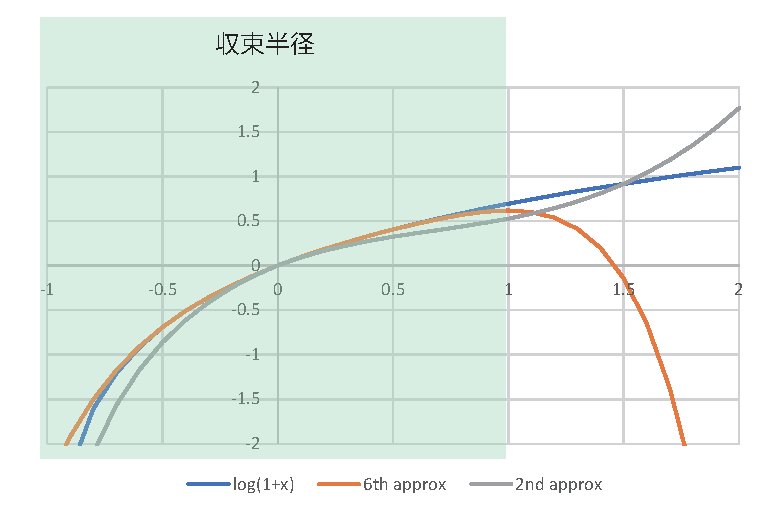
\includegraphics[width=8cm]{calculus9/roc.eps}
\end{figure}
マクローリン級数の次数を多くすると、収束半径内では近似が改善、収束半径外では近似が発散している。
(roc.xlsx参考)

\end{slide}


%%%%%%%%%%%%%%%%%%%%%%%%%%%%%%%%%%%%%%%%%%%%%%%%%%%%%%%%%%%%%%%%%%%%%%%%%%%%%%%%%%%%%%%
%%%%%%%%%%%%%%%%%%%%%%%%%%%%%%%%%%%%%%%%%%%%%%%%%%%%%%%%%%%%%%%%%%%%%%%%%%%%%%%%%%%%%%%



\section{今日のまとめ}
\begin{frame}
\frametitle{まとめ}   


\begin{enumerate}
\item テイラーの定理の証明
\item テイラー展開, 解析的関数
\item 応用, オイラーの公式
\item 収束半径
\end{enumerate} 

\end{frame}
\begin{slide}{課題 \#9}
$f(x)=\cos(x)$の定義域を$-10 \le x \le 10$とし、二次までのマクローリン展開した場合、$\pm$1.5ラジアンを超えた付近から、下図のように近似精度が急速に劣化してしまう。級数の打ち切り次数を増やすことによって定義域$-10 \le x \le 10$全体で、近似できるか、できないか回答しなさい。もしで近似できると考える場合には、概ね何次まで級数展開すれば良好な近似が与えられるか図を用いるなどして説明せよ。

\begin{figure}[h]
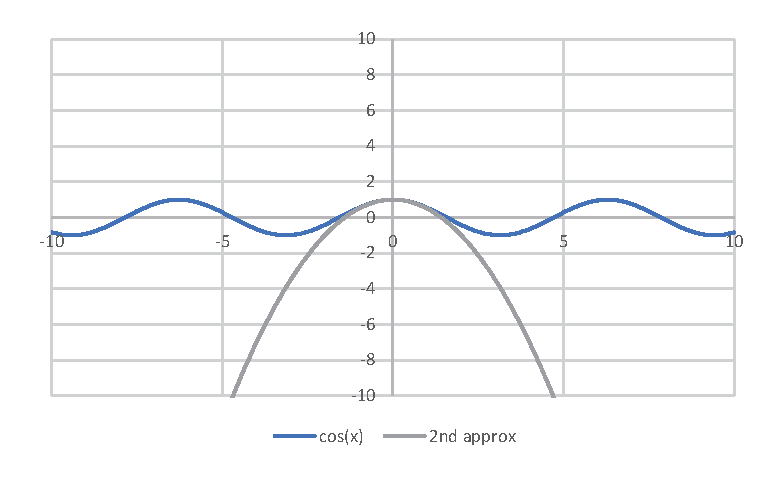
\includegraphics[width=8cm]{calculus9/roccos.eps}
\end{figure}


\end{slide}
